\section[Introdução]{Introdução}

\begin{frame}
  \frametitle{Introdução}
  \begin{itemize}
    \item Gerenciamento e manutenção de arquivos: desafio;
          \begin{itemize}
            \item backups não realizados;
            \item sobrescrita de arquivos;
            \item difícil manutenabilidade em times;
          \end{itemize}
    \item Diferentes soluções no mercado: \textit{CVS}, \textit{Subversion}, \textit{TFS}, \textit{Mercurial}.
  \end{itemize}
\end{frame}

\begin{frame}
  \frametitle{GitHub}
  \begin{itemize}
    \item \textit{Git} + \textit{GitHub} = \textit{OpenSource}.
    \item \textit{GitHub} que é uma plataforma para versionamento, gerenciamento e colaboração de projetos, que utiliza o \textit{Git} como base. \cite{Scott:ProGit}
  \end{itemize}
\end{frame}

\begin{frame}
  \frametitle{Controle de Issues}
  \begin{itemize}
    \item Dentre outras ferramentas temos o controle de \textit{Issues:}.
          \begin{itemize}
            \item documentar possíveis \textit{bugs}, melhorias, ou novas \textit{features} para os projetos
          \end{itemize}
  \end{itemize}
\end{frame}

\begin{frame}
  \frametitle{Exemplo Issues}
  \begin{figure}[htbp]
    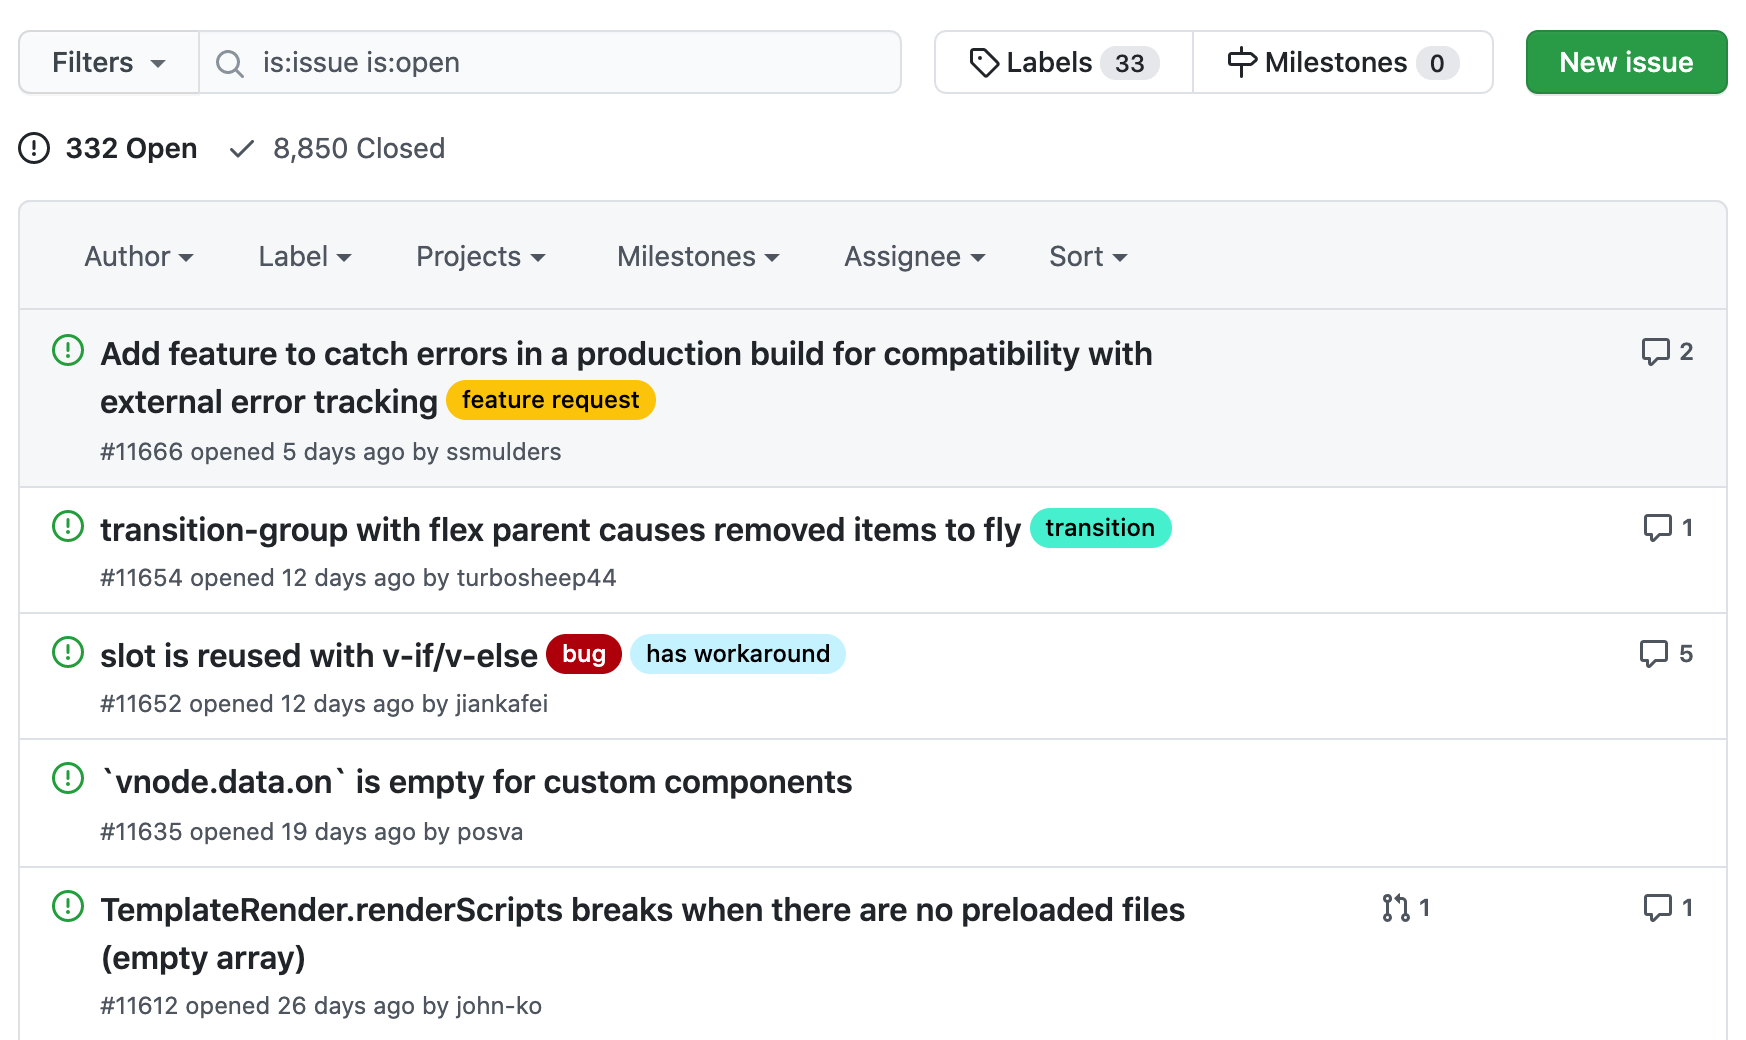
\includegraphics[width=\textwidth]{images/issues_example.png}
    \caption{Exemplos de Issues do Projeto Vue.js}
  \end{figure}
\end{frame}

\begin{frame}
  \frametitle{Issues sobre Segurança}
  \begin{itemize}
    \item Eventualmente, as \textit{issues} podem estar relacionadas a tópicos de segurança.
    \item Quando consideradas críticas, podem ser analisadas por outros especialistas;
    \item Como identificar quais \textit{issues} que são relacionadas com segurança?
    \item Como classificar estas \textit{issues} para que especialistas possam analisar os cógidos?
  \end{itemize}
\end{frame}

\begin{frame}
  \frametitle{Proposta do Trabalho}
  \begin{itemize}
    \item Criação de uma ferramenta que utilize técnicas de \textbf{aprendizagem de máquina} para o desenvolvimento de um classificador que consiga analisar as palavras contidas nas mensagens das \textit{issues} de um dado projeto, e classificar se esta \textit{issue} está ou não relacionada no contexto de segurança da informação.
  \end{itemize}
\end{frame}